%este arquivo contém todas as seções do capítulo de introdução

A ascensão de novos modelos de negócio está redefinindo o setor da beleza no Brasil, impulsionando a autonomia de seus profissionais. Entre as inovações mais significativas, destaca-se o \emph{coworking} de beleza, que transforma a dinâmica de trabalho ao oferecer infraestrutura compartilhada e flexível. Esse formato libera cabeleireiros, maquiadores e outros especialistas da necessidade de arcar com os altos custos de um salão próprio, de depender de parcerias em estabelecimentos de terceiros ou atender à domicílio \cite{BeautyFair, gazeta-coworking}. 

Essa modernização ocorre em um mercado robusto, que movimentou aproximadamente US\$\,27\,bilhões em 2024 e posicionou o país entre os cinco maiores do mundo no ramo, evidenciando a necessidade de adaptação contínua dos empreendedores às novas tendências \cite{Sebrae_2024}. Contudo, à medida que esse formato de trabalho se expande, a gestão eficiente de agendas, espaços e custos torna-se um desafio central para maximizar a autonomia e a rentabilidade. A necessidade de evitar conflitos de reserva e falhas de cobrança de forma ágil e intuitiva é cada vez mais necessária.

Este projeto propõe-se, portanto, a desenvolver uma aplicação web que atenda exatamente a essa demanda.

\section{Objetivos}

A aplicação \emph{web} BS Beauty foi desenvolvida especialmente para gerenciar um salão de beleza que opera em modelo \emph{coworking}, sob a gestão de nossa parceira de extensão Bruna. Seu objetivo principal é otimizar os processos internos e centralizar o agendamento de serviços, atendendo tanto às demandas da gestora quanto às necessidades dos profissionais autônomos.

\noindent\textbf{Para os Clientes Finais:} A plataforma possibilita o agendamento de serviços de forma intuitiva e flexível. Os clientes poderão escolher profissionais específicos ou optar pelo melhor horário disponível, visualizando facilmente a lista de prestadores, seus serviços, preços, tempo de execução e agendas atualizadas.

\noindent\textbf{Para os Profissionais Autônomos:} O sistema BS Beauty tem como propósito reforçar a autonomia dos profissionais sobre sua agenda e finanças. A aplicação permite bloquear horários, editar preços e a duração dos serviços, além de acompanhar os agendamentos realizados (sejam eles do dia, futuros ou passados) e visualizar relatórios detalhados com a receita gerada pelos serviços prestados.

\noindent\textbf{Para a Gestora:} Nossa parceira, Bruna, terá acesso a funcionalidades exclusivas que incluem análise de métrica de desempenho (a partir de \emph{dashboards)}, gerenciamento do aluguel ou comissão de cada profissional, visualização do fluxo de agendamentos em períodos específicos, envio de mensagens de \emph{marketing} e promoções aos clientes, e acesso a relatórios financeiros detalhados. Ademais, a gestora poderá incluir ou remover profissionais da plataforma conforme a necessidade.
\section{Problema e Solução Proposta}

A gestão de um salão por pequenos empreendedores é frequentemente desafiadora. Ademais, demandas surgem e muitas vezes são realizadas manualmente. Portanto, quando alguma etapa falha, evidencia‐se a necessidade de uma solução digital capaz de reduzir erros e diminuir o esforço administrativo.

Por isso, o objetivo geral do projeto é suprir as necessidades de um salão de beleza em modelo \emph{coworking} de forma ágil. Como explicado anteriormente, esse modelo de trabalho é recente (popularizado após a pandemia de \gls{covid} em 2020) e atende diferentes profissionais autônomos (relacionados à gerente por locação ou comissão), não uma equipe com objetivo comum. Desta forma, o problema central é gerenciar a ocupação de cada profissional no espaço de trabalho, além de controlar as finanças e a agenda de clientes.

Nossa parceira Bruna já utilizava um sistema digital para gerenciamento do salão. Contudo, apesar dos benefícios trazidos pela solução, o sistema apresentava pontos insatisfatórios, sendo o principal deles a instabilidade da plataforma, que gerava insatisfação e perda de clientes.

Nossa solução consiste em criar uma aplicação \emph{web} que mantenha todas as funcionalidades que já atendem bem a Bruna como o agendamento \emph{on-line} e pesquisa de satisfação. Além disso, a plataforma incluirá funções ainda ausentes e ajustará requisitos funcionais e não funcionais cuja concepção é adequada, mas apresenta falhas, como o \emph{login} instável, senhas excessivamente complexas e erros recorrentes na troca de senha.

Em síntese, a solução proposta é uma plataforma com \emph{login} simplificado (integrado ao \gls{sso} \footnote{Single Sign-On é um sistema que permite usar um único nome de usuário e senha para acessar vários serviços diferentes, sem precisar criar contas ou lembrar várias senhas.} do Google) e agendamento fácil e transparente para os clientes (incluindo todos os serviços e atributos necessários para uma melhor decisão). Também contará com agenda totalmente controlada pelos profissionais, notificações de agendamento e cancelamento para clientes e profissionais, lista de aniversariantes, desconto por frequência e retenção de dados em conformidade com a \gls{lgpd}. Além disso, a gerente terá acesso à relatórios financeiros e \emph{dashboards} com métricas de produtividade e frequência de clientes.

\section{Justificativa}

Uma pesquisa de 2023 do SEBRAE indica mais de 1,3 milhão de atividades econômicas ligadas a negócios de beleza no Brasil, abrangendo serviços, indústria e comércio, e gerando aproximadamente R\$ 75 bilhões em faturamento anual \cite{sebrae2023forca}. O gráfico abaixo (figura \ref{fig:profissionais_brasil}) demostra o crescimento da quantidade de profissionais no setor da beleza nos últimos anos:

 \begin{figure}[htb]
 	\centering
 	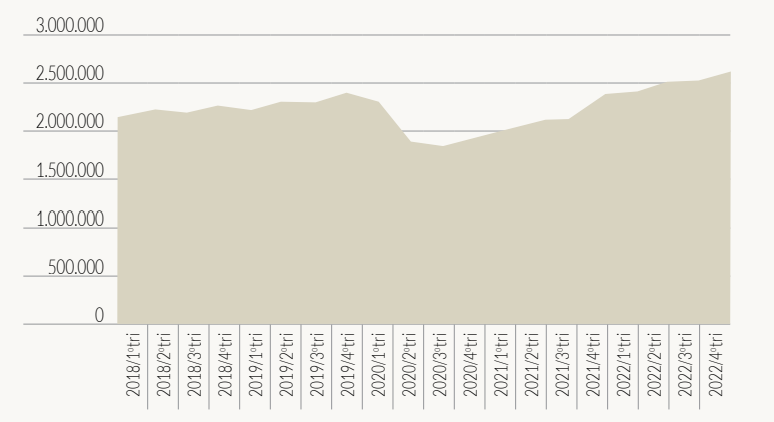
\includegraphics[width=0.9\textwidth]{cap01-Introducao/Images/1.3_grafico_profissionais_brasil}
 	\caption{Profissionais da área da beleza no Brasil 2018–2022}
 	\label{fig:profissionais_brasil}
 	\fonte{\cite{senac_panorama_mercado}}
 \end{figure}
 
 \FloatBarrier
 
Embutido neste crescimento, a maior parte dos profissionais são cabeleireiros, como mostra o gráfico abaixo (\ref{fig:Distribuição_profissionais})

%inicio de figura
\begin{figure}[htb]
	\centering
	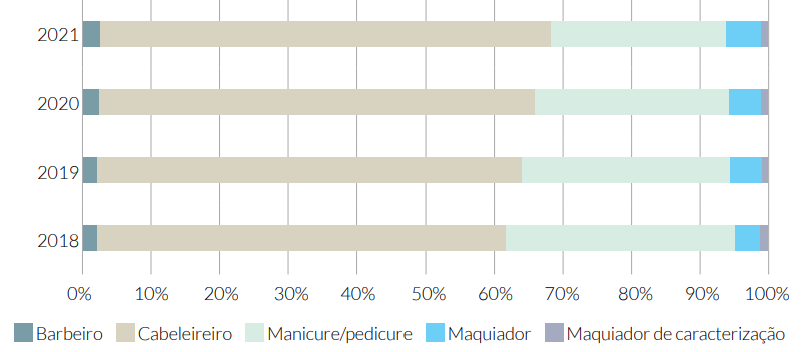
\includegraphics[width=0.9\textwidth]{cap01-Introducao/Images/1.3_grafico_maioria_cabeleireiros}
	\caption{Distribuição dos profissionais da área da beleza 2018-2021}
	\label{fig:Distribuição_profissionais}
	 \fonte{\cite{senac_panorama_mercado}}
\end{figure}

\FloatBarrier

Neste cenário robusto, que movimentou cerca de 27 bilhões de dólares em 2024 \cite{ecommercenapratica2025}, os desafios operacionais crescem cada vez mais: 

\begin{itemize}
	\item Até 30\% do tempo de um pequeno empreendedor é consumido por tarefas administrativas \cite{senac2022};
	\item Taxa média de não comparecimento de clientes atinge 25\% \cite{booksy2022};
	\item Perda de 20\% da receita por não comparecimento \cite{abihpec2021};
	\item Média de 15 horas semanais dedicadas ao controle manual de agenda e finanças \cite{fgv2020};
	\item Insatisfação de 40\% dos clientes devido a falhas de comunicação e alterações de última hora \cite{mindminers2022}.
\end{itemize}

Paralelamente ao crescimento do setor de beleza, o modelo de \emph{coworking}, originado em ambientes de escritório, expandiu-se para salões, permitindo o compartilhamento de espaços e recursos e a redução de custos \cite{sebrae_coworking,sebraesc2025}. Anteriormente à população dos \emph{cowrokings} de beleza, os profissionais se distribuiam em diversos locais para economizar recursos, como mostra a figura \ref{fig:Distribuição_locais}

%inicio de figura
\begin{figure}[htb]
	\centering
	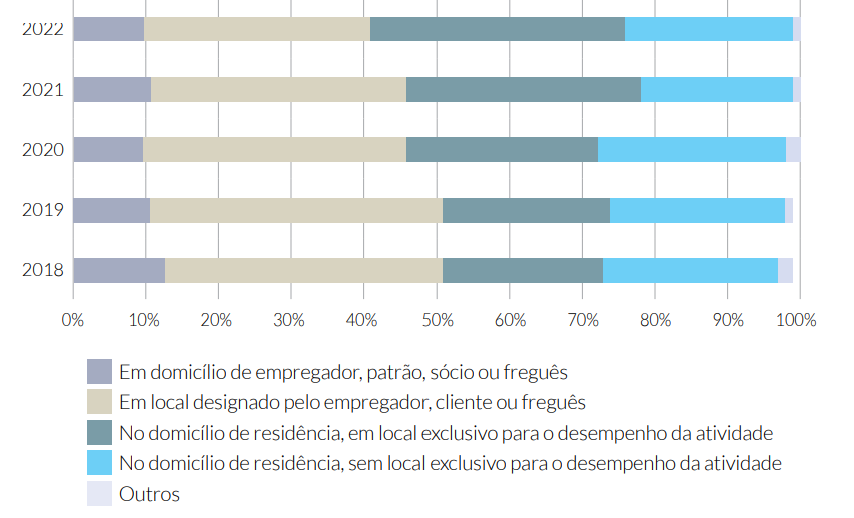
\includegraphics[width=0.9\textwidth]{cap01-Introducao/Images/1.3_local_trabalho_profissionais}
	\caption{Distribuição dos profissionais da área da beleza por local de trabalho 2018-2022}
	\label{fig:Distribuição_locais}
	\fonte{\cite{senac_panorama_mercado}}
\end{figure}

\FloatBarrier

Nesse contexto promissor, justifica-se o projeto de extensão \emph{BS Beauty}, destinado a desenvolver uma aplicação web customizada para o gerenciamento de salões em modelo coworking, sob a coordenação de nossa parceira de extensão Bruna. Ao digitalizar e centralizar processos principais, a BS Beauty empodera pequenos empreendedores reduzindo custos operacionais e minimizando erros humanos, melhora a experiência do cliente, eleva a receita dos profissionais por meio do controle preciso de comissões e frequências, e oferece a oportunidade de \emph{insights} estratégicos através de dashboards e relatórios financeiros detalhados. 

Dessa forma, a solução não só supera os problemas de instabilidade e excesso de esforço administrativo, mas também gera valor para todos os envolvidos no salão de beleza. Além disso, como iniciativa de extensão, o projeto permite que os alunos‐desenvolvedores coloquem em prática e melhorem os conhecimentos técnicos e de gestão,  aprendendo com desafios reais de requisitos, usabilidade e performance. Assim, é possível aproximar a graduação das demandas do mercado.



\section{Análise da Concorrência}

Foi conduzida uma pesquisa de mercado centrada em plataformas brasileiras que combinam agendamento on-line e gestão financeira para espaços de beleza no modelo \emph{coworking}. Deste levantamento emergiram três empresas que servirão de referência nesta análise: uma já amplamente consolidada no mercado nacional — embora atue além do universo \emph{coworking} — e outras duas que, apesar de conhecidas, ainda estão em expansão, mas com foco mais relacionado ao da nossa proposta, o que as torna concorrentes que merecem maior atenção estratégica.

\subsection{Trinks}

%inicio de figura
\begin{figure}[htb]
	\centering
	
\includegraphics[width=0.5\textwidth]{cap01-Introducao/Images/1.4.1_Trinks}
	\caption{Logo plataforma Trinks}
	\label{fig:Trinks}
\end{figure}

 \FloatBarrier

Trinks é uma plataforma já bem consolidada no mercado de gestão de negócios de beleza, com soluções
personalizadas para barbearias, salões de beleza e clínicas de estética. Criada em 2012, é hoje a
plataforma de gestão para beleza com a maior base instalada do país, englobando aproximadamente
2,8\,milhões de usuários e mais de 40\,mil estabelecimentos, sediada no Rio de Janeiro. A plataforma começou como um empreendimento de consultoria em software personalizado, mas logo identificou uma oportunidade no mercado da beleza e mudou de nicho. Em 2024, foi adquirida pelo grupo Stone, o que alavancou ainda mais funcionalidades do aplicativo, como o autoatendimento.
Atualmente, a Trinks oferece software de back-office (conjunto de módulos internos que controlam o funcionamento do negócio como finanças, estoque, comissões e relatórios), marketplace B2C e meios de pagamento próprios (Trinks Pay), funcionando praticamente como um “ERP + iFood” para salões e barbearias. Existe um
plano grátis que engloba apenas 150 agendamentos por mês, e os planos pagos variam de R\$ 59 a R\$ 249/mês \cite{Trinks}.

Além dos serviços comuns, seus principais diferenciais são:

\begin{itemize}
	\item Ponto de venda (PDV) completo: integração TEF, Pix e split de comissão, atendendo desde
	MEIs até redes com exigência de NFC-e e SAT/ECF;
	\item Marketplace \textit{Trinks.com}, que gera maior fluxo de clientes, expõe o salão ao
	público final e permite pagamento antecipado;
	\item Estrutura em nuvem madura, com SLA de 99{,}9\,\% e aplicativos nativos para
	iOS/Android.
\end{itemize}

Apesar dos grandes benefícios, identificamos algumas brechas do ponto de vista do negócio da nossa
parceira de extensão, Bruna:

\begin{itemize}
	\item A interface pode ser considerada “poluída” para clientes iniciantes, devido ao grande
	número de funcionalidades;
	\item Há pouco foco no aluguel de estações típico do coworking, exigindo ajustes manuais de
	comissão;
	\item Maior parte das funcionalidades estão presentes apenas nos planos superiores.
\end{itemize}

\subsection{Gendo}

%inicio de figura
\begin{figure}[htb]
	\centering
	
\includegraphics[width=0.4\textwidth]{cap01-Introducao/Images/1.4.2_Gendo}
	\caption{Logo plataforma Gendo}
	\label{fig:Gendo}
\end{figure}

 \FloatBarrier

Lançado em 2017 e sediado em Curitiba-PR, o Gendo se posiciona como um \emph{hub}\footnote{Hub: plataforma centralizada que integra agenda, PDV, finanças e pagamentos em um único ambiente, funcionando como “nó” que organiza os fluxos de dados do negócio.} de gestão 100\,\% em nuvem para negócios além do setor da beleza, como estética, saúde, bem-estar, pet-shop e mais recentemente, espaços em formato coworking. 
Atualmente mantém mais de 10 mil assinantes, com maior penetração nas regiões Sul e Sudeste do Brasil. Foi criado no modelo SaaS com o intuito de oferecer prontamente agenda on-line, automação de lembretes (e-mail/WhatsApp), módulo financeiro completo e integrações com gateways de pagamento (Stone, Cielo e Mercado Pago). Atualmente, os planos são somente pagos e variam de R\$ 32 a R\$ 293/mês, após 14 dias de teste gratuito \cite{Gendo}.

Seus principais diferenciais são:
\begin{itemize}
	\item Caixa do profissional: Módulo pensado para coworking, possibilitando débito automático de aluguel de estação e visualização dos ganhos de cada profissional;
	\item Aplicativo Gendo Pro (iOS e Android): permite ao profissional ver a agenda, acompanhar comissões, pedir saques e registrar fotos de antes e depois dos serviços;
	\item Relatórios instantâneos: exibem ticket médio, previsão de faturamento e dados de cancelamentos, com opção de exportar para Excel.
\end{itemize}


Já os maiores pontos de melhoria identificados são:
\begin{itemize}
	\item Base instalada ainda pequena, limitando o efeito de rede junto a grandes franquias;
	\item Dependência de gateways externos, o que adiciona custo extra ao \emph{split} \footnote{Split é a divisão automática do pagamento entre salão e profissional que, se feita por um gateway externo, gera uma taxa extra.};
	\item Relatórios fiscais avançados disponíveis apenas no plano Premium.
\end{itemize}

\subsection{Avec}

\begin{figure}[htb]
	\centering
	
\includegraphics[width=0.4\textwidth]{cap01-Introducao/Images/1.4.3_Avec}
	\caption{Logo plataforma Avec}
	\label{fig:Avec}
\end{figure}

 \FloatBarrier

A Avec é, hoje, a principal concorrente do nosso projeto, pois a entidade parceira que motivou este trabalho utiliza essa plataforma para gerenciar seu salão de beleza em modelo coworking. Por esse motivo, ela foi adotada como referência: buscamos manter as funcionalidades que já funcionam bem na Avec e, ao mesmo tempo, acrescentar ou aprimorar recursos que ainda fazem falta para a nossa parceira.

Lançada em 2014 e sediada em São Paulo-SP, a Avec se apresenta como solução``360º'' para salões, barbearias, esmaltarias, spas e estúdios de tatuagem. A plataforma integra software de gestão, um sistema próprio de pagamentos (\emph{Avec Pay}) e um marketplace B2C que encaminha novos clientes aos estabelecimentos. Segundo a empresa, mais de 40 mil negócios utilizam o serviço no
Brasil. Também desenvolvida no modelo SaaS, a ferramenta oferece agenda on\-/line multiprofissional com confirmações via WhatsApp ou SMS, ponto de venda completo com TEF, Pix e \emph{split} interno de comissões, além de módulo financeiro integrado. Dispõe ainda de uma carteira digital empregada em pacotes pré\=/pagos, gift-cards
e cashback, e de dois aplicativos: o \emph{Avec}, voltado ao cliente final, e o \emph{Avec Pro}, destinado aos profissionais. Há um plano gratuito ``\emph{Avec Go}'' que inclui funções básicas e cobra apenas a taxa transacional, enquanto os planos pagos variam de R\$ 77 a
R\$249 por mês \cite{Avec}.


Com base no feedback da nossa entidade parceira, destacam-se quatro funcionalidades que
a plataforma \emph{Avec} executa bem:
\begin{itemize}
	\item \emph{Split} instantâneo de comissões, dispensando gateways externos;
	\item Marketplace B2C e aplicativo do cliente, que ampliam a visibilidade do salão e aumentam os agendamentos on-line;
	\item App \emph{Avec Pro} (iOS/Android), no qual o profissional acompanha agenda,
	comissões, saques e registra fotos de “antes e depois” dos serviços.
\end{itemize}

As principais brechas identificadas são:
\begin{itemize}
	\item módulos fiscais avançados (NF-e e SAT) disponíveis apenas nos planos superiores;
	\item dependência do hardware e das tarifas do próprio \emph{Avec Pay} para uso pleno do sistema;
	\item custos adicionais para envios em massa de SMS/WhatsApp em campanhas de marketing;
	\item instabilidade recorrente: o domínio eventualmente fica fora do ar.
\end{itemize}

%seção 1.4 quadro comparativo

\subsection{Quadro comparativo}

\begin{quadro}[htb]
	\caption{\label{frame:comparativo_concorrência}Comparação entre as plataformas concorrentes e a aplicação proposta}
	\footnotesize
	\setlength{\tabcolsep}{4pt}
	\begin{tabular}{|p{6.8cm}|c|c|c|c|}
		\hline
		\textbf{Recurso}                                   & \textbf{Trinks} & \textbf{Gendo} & \textbf{Avec} & \textbf{BS Beauty}\\ \hline 
		Aplicação \textit{web}  & — & \checkmark & \checkmark & \checkmark \\ \hline
		Foco no coworking  & — & \checkmark & — & \checkmark \\ \hline
		Controle de acesso para gestão  & — & \checkmark  & \checkmark & \checkmark \\ \hline
		Agendamento de serviços 100\% on-line & \checkmark & \checkmark & \checkmark & \checkmark \\ \hline
		Controle de conflitos de agenda                    & \checkmark & \checkmark & \checkmark & \checkmark \\ \hline
		Avaliação pós-serviço  & \checkmark & \checkmark  & \checkmark  & \checkmark \\ \hline
		Plataforma do \textit{cliente}                               & \checkmark & \checkmark & \checkmark & \checkmark \\ \hline
		Plataforma do \textit{profissional}                                        & \checkmark & \checkmark & \checkmark & \checkmark \\ \hline
		Confirmação automática (WhatsApp / SMS / e-mail)                    & \checkmark & \checkmark & \checkmark & \checkmark \\ \hline
		Cálculo de \emph{Split} de comissão      & \checkmark & \checkmark & \checkmark & — \\ \hline
		Pagamento on-line                 & \checkmark & — & \checkmark & \ — \\ \hline
		Marketplace B2C                         & \checkmark & — & \checkmark & \ — \\ \hline
		Marketing integrado (envio em massa de SMS/WhatsApp/e-mail)  & \checkmark & — & \checkmark & \checkmark \\ \hline
		Gift-card                     & \checkmark & — & \checkmark & \checkmark \\ \hline
		Programa de indicação  & \checkmark & — & \checkmark & \checkmark \\ \hline
		Relatório financeiro em tempo real    & \checkmark & \checkmark & \checkmark & \checkmark \\ \hline
		Login simplificado com integração Google            & \checkmark & \checkmark &  — & \checkmark \\ \hline
		Plano gratuito disponível                                           & \checkmark & — & \checkmark & \checkmark \\ \hline
		Lista de aniversariantes para promoções  & \checkmark & \checkmark & — & \checkmark \\ \hline
		
	\end{tabular}
	\fonte{Produzido pelos autores}
\end{quadro}

